\documentclass[conference]{IEEEtran}

\usepackage{cite}
\usepackage{graphicx}
\usepackage{tabularx, booktabs}
\usepackage{subfig}
\hyphenation{op-tical net-works semi-conduc-tor}

\newcommand{\Comment}[1]{\textbf{#1}}


\begin{document}

\title{Performance Analysis of CNN Frameworks\\
 for GPUs}

%\author{\IEEEauthorblockN{Heehoon Kim$^{*\ddagger}$ $\quad$ Hyoungwook
%    Nam$^{\dagger\ddagger}$ $\quad$ Wookeun Jung$^*$ $\quad$ Jaejin Lee$^*$}\\
%\IEEEauthorblockA{$^*$Department of Computer Science and Engineering,\\
%$^\dagger$Department of Computer Science and Engineering,\\
%Seoul National University, Korea\\
%{\texttt \{heehoon, hyoungwook,
%  wookeun\}@aces.snu.ac.kr,jaejin@snu.ac.kr}\\
%http://aces.snu.ac.kr}\\
%$^{\ddagger}$These two authors contributed equally to this work
%      as the first authors.
%}

\maketitle

\begin{abstract}
Thanks to modern deep learning frameworks that exploit GPUs, convolutional neural networks (CNNs) have been greatly successful in visual recognition tasks. In this paper, we analyze the GPU performance characteristics of five popular deep learning frameworks: Caffe, CNTK, TensorFlow, Theano, and Torch in the perspective of a representative CNN model, AlexNet. We identify the overhead of each framework and suggest possible optimization methods to increase the efficiency of CNN models built by the framework. We also show the GPU performance characteristics of four convolution algorithms each of which uses one of GEMM, direct convolution, FFT, and Winograd method. Based on the characterization, we suggest criteria to choose convolution kernels for GPUs and methods to build efficient CNN models on GPUs. Since scaling DNNs in a multi-GPU context becomes important, we also analyze the scalability of the deep learning frameworks in the multi-GPU context and their overheads. Based on the multi-GPU characterization, we suggest possible optimization methods for CNNs in the multi-GPU context.
\end{abstract}

\IEEEpeerreviewmaketitle

\section{Introduction}

Deep neural networks (DNNs) have been very successful on various machine learning tasks, such as visual recognition\cite{krizhevsky2012imagenet,vgg,RCNN}, speech recognition\cite{speech}, and machine translation\cite{machinetranslation}.
Among others, the convolutional neural network (CNN) proposed by LeCun \textit{et al.}\cite{726791}, is one of the earliest successful DNN models that were used to classify images.
CNN models equipped with deep learning techniques (\textit{e.g.}, ReLU activation, dropout layers, data augumentation, etc.) outperform previous machine learining techniques in various visual recognition challenges, such as ILSVRC\cite{DBLP:journals/corr/RussakovskyDSKSMHKKBBF14} and PASCAL\cite{pascal}.
The classification accuracy of CNN models have been improving over time.
In addition, recent state-of-the-art techniques for visual recognition use an ensemble of different CNN models\cite{ILSVRC15}.
CNN models are also being applied to other machine learning tasks than image recognition.
They can also be applied to action recognition\cite{actionrecognition}, speech recognition\cite{speech}, natural language processing\cite{DBLP:journals/corr/KalchbrennerGB14}, and playing Go\cite{alphago}.

The biggest advantage of using DNN is its scalability.
A larger and deeper DNN with more parameters usually results in a better accuracy.
However, a larger DNN require more processing power, and training it using a typical computer is impractical.
Fortunately, computations in a neural network can easily be represented as tensor or matrix operations that can be efficiently parallelized.
Thus, GPUs' massively parallel processing power make DNNs to be trained efficiently even in a single desktop computer.
Since deep learning frameworks have been developed for the efficient and easy implementation of DNN models, most of popular deep learning frameworks support GPU acceleration by default\cite{DBLP:journals/corr/Al-RfouAAa16,jia2014caffe,tensorflow2015-whitepaper,torch,cntk}.
As a result, companies and researchers have been trying to implement efficient GPU kernels to improve the performance of deep learning frameworks.

The most popular deep learning library for such frameworks is cuDNN\cite{cudnn}.
It has been developed by NVIDIA, and most of the popular deep learning frameworks use it as the backend for GPUs.
For example, computing convolution with cuDNN results in up to 4X performance improvement compared with the default GPU kernels of the frameworks\cite{convnet-benchmarks}.
Another approach to speed up CNNs is reducing the time complexity of convolution algorithms.
Fast Fourier Transform (FFT) algorithms\cite{fftconv, fbfft} and Winograd's minimal filtering algorithm\cite{winograd} successfully reduce the time complexity of the convolution computation.
However, while the efficiency of deep learning on a single GPU has been improved a lot, deep learning on multiple GPUs still shows poor scalability\cite{DBLP:journals/corr/YadanATR13}.

In this paper, we analyze the performance characteristics of CNNs on different deep learning frameworks and libraries.
For clarity, a \textit{framework} refers to a full collection of libraries to build DNN models and a \textit{library} refers to a GPU kernel library such as cuDNN used for the framework.
We choose five most popular deep learning frameworks, Caffe\cite{jia2014caffe}, CNTK\cite{cntk}, TensorFlow\cite{tensorflow2015-whitepaper}, Theano\cite{DBLP:journals/corr/Al-RfouAAa16}, and Torch\cite{torch}.
The criterion for popularity is the number of github\cite{github} stars.
We also choose a CNN model, AlexNet\cite{krizhevsky2012imagenet}, to obtain the performance characteristics from the frameworks and libraries.
Identically structured AlexNet models are built and trained using these frameworks.
All the five frameworks use cuDNN as the GPU backend.
Cuda-convnet\cite{cuda-convnet} developed by Alex Krizhevsky is another GPU library used in this paper.
In addition, we compare three different convolution algorithms of cuDNN with the direct convolution algorithm of cuda-convnet.

The contributions of this work can be divided into three parts.
First, we analyze differences in the performance characteristics of the frameworks.
We identify performance limiting factors of each framework and describe pros and cons of using each deep learning framework for propspective users.
The performance limiting factors would also be helpful to optimizing the frameworks.
Second, we obtain the performance characteristics of different convolution algorithms.
Based on the result of analyzing the charateristics, we provide possible optimization techniques to implement efficient CNN models using the libraries.
Finally, we obtain the performance characteristics of the frameworks in multi-GPU contexts. We also provide possible techniques to improve the scalability of the frameworks when using multiple GPUs.

\section{Background and Related work}

\subsection{Previous work}
It has been only a few years since deep learning frameworks were introduced to public.
Few attempts recently tried to benchmark and compare the performance of the frameworks.
A benchmark of CNN frameworks is publicly available on Github\cite{convnet-benchmarks}.
It shows forward and backward propagation time of CNN model for each framework.
But the latest result was tested with cuDNN version R4, while the most recent version is R5.1.
Detailed benchmarks of deep learning frameworks were recently published\cite{DBLP:journals/corr/BahrampourRSS15, DBLP:journals/corr/ShiWXC16}.
They show execution times of various DNN models run on the frameworks.
However, the benchmarks show only the results, without identifying the reasons for the differences.
They also use cuDNN version of R4, which do not support most recent Winograd convolution.


\subsection{Machine learning frameworks}

Theano is a python framework for evaluating mathematical expressions\cite{DBLP:journals/corr/Al-RfouAAa16}.
It is one of the earliest framework used to build DNN models.
Multiple machine learning frameworks are built on top of Theano.
Pylearn2, Keras and Lasagne are popular frameworks for DNN using Theano as their backend.
Multiple GPU support of Theano is still on experimental stage.
Torch is a scientific computing framework based on LuaJIT\cite{torch}.
Torch is also one of the earliest frameworks used to implement CNN models.
Nvidia's self-driving car project and Deepmind's Deep Q Learning model were built on Torch\cite{nvdave, mnih2015humanlevel}.
Torch natively supports multi-gpu context via its cutorch module.
Caffe is deep learning framework developed by Berkeley Vision and Learning Center\cite{jia2014caffe}.
Caffe use prototxt file to describe DNN models.
Pre-trained network models can be imported with prototxt files.
Visual recognition challenge winners are usually implemented by Caffe\cite{ILSVRC15, RCNN, vgg}.
The flexibility of Caffe is limited.
Introducing a new feature to a layer requires re-building of the entire source code.
The multi-gpu support of Caffe is limited to batch data parallelism.
Tensorflow is machine learning framework developed by Google\cite{tensorflow2015-whitepaper}.
It was first introduced to public in 2015, and is now the most popular machine learning framework on GitHub.
Tensorflow supports both Python and C++ interface.
Computational Network Toolkit(CNTK) is deep learning framework developed by Microsoft\cite{cntk}.
CNTK supports both Windows and Linux environment, while the others do not support Windows.
CNTK uses its own BrainScript to describe DNN models.
It also supports C++ and C\# wrappers to evaluate models.

\begin{figure}
  \centering
  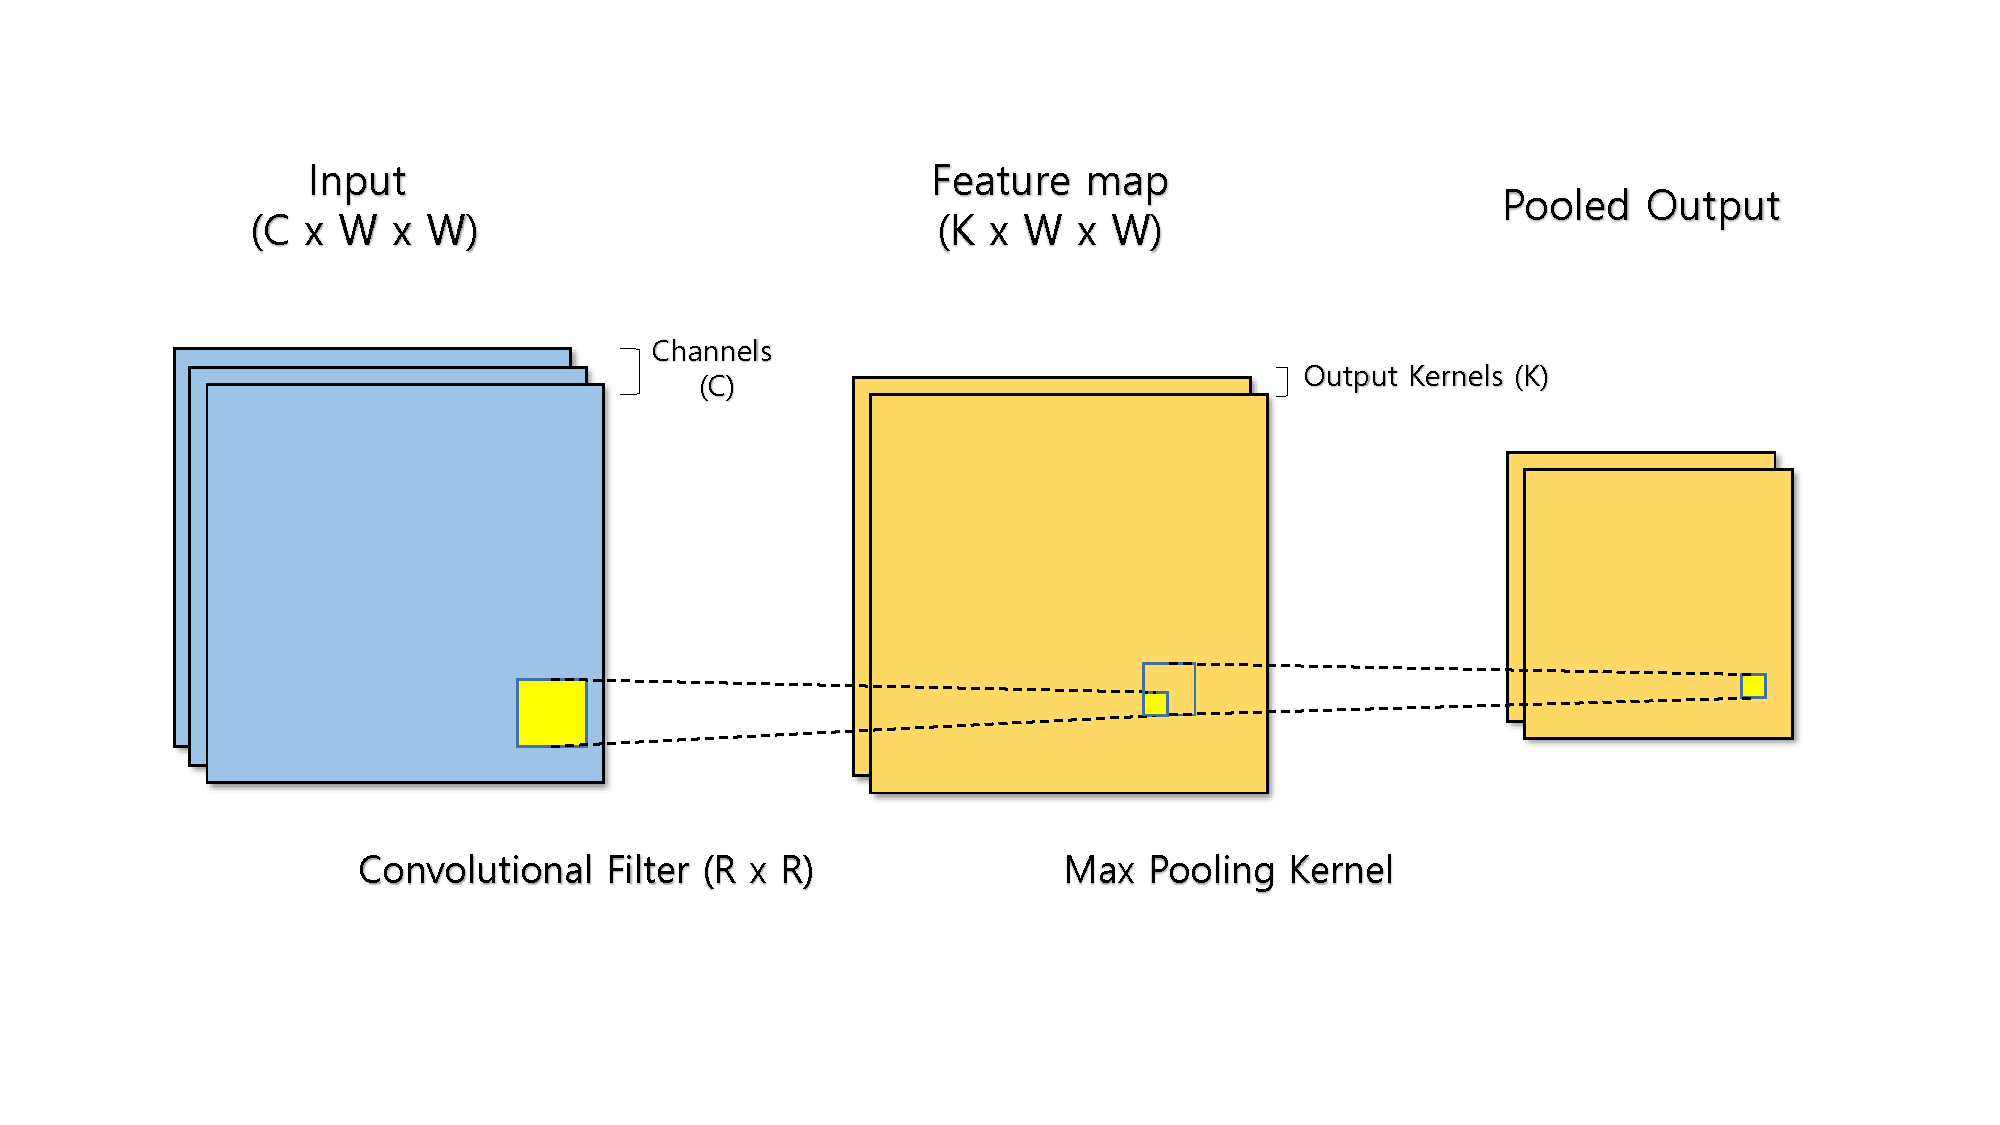
\includegraphics[width=\linewidth]{./figures/conv_2dlayer}
  \caption{An example of typical 2D convolution layer. }
  \label{fig_convlayer}
\end{figure}
\begin{figure}
  \centering
  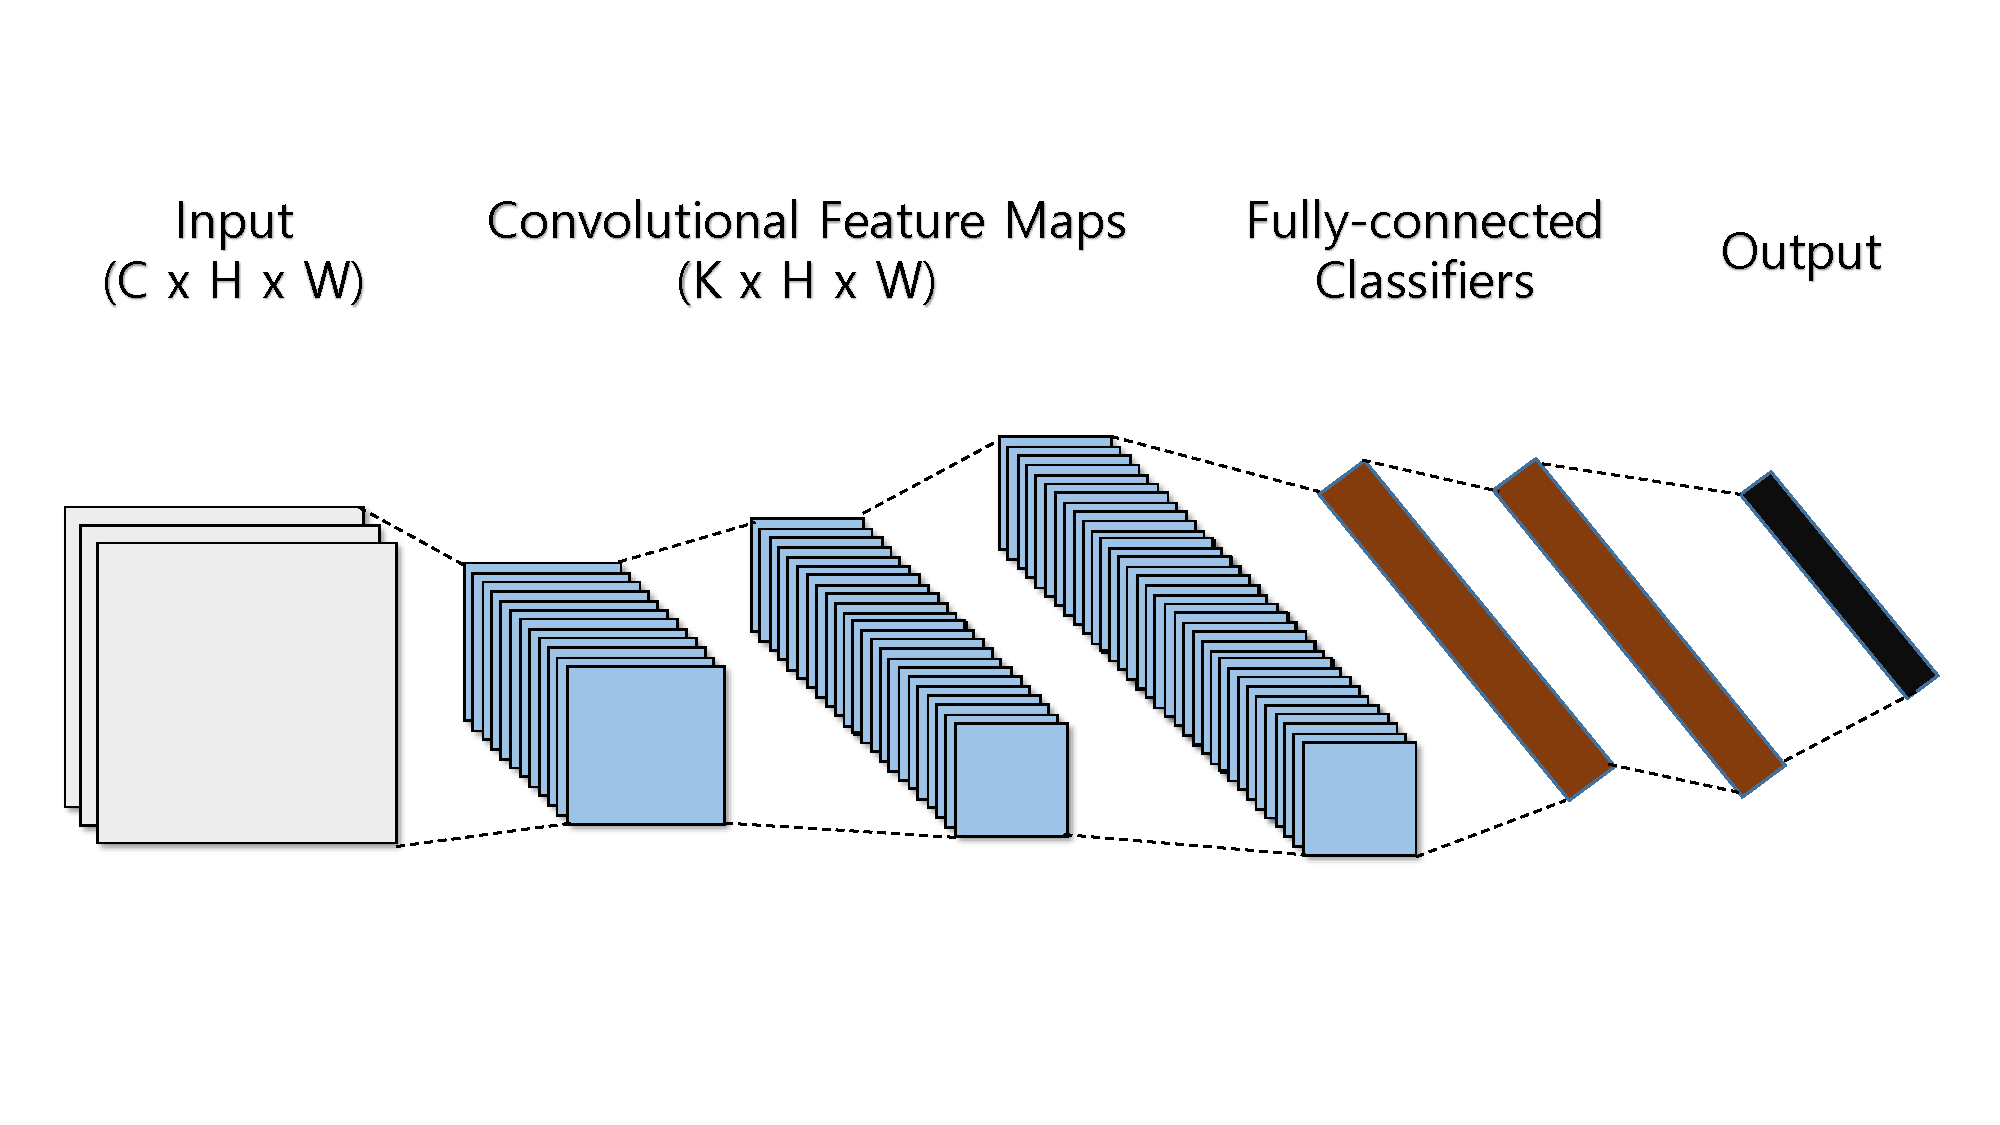
\includegraphics[width=\linewidth]{./figures/conv_model}
  \caption{A typical CNN network model }
  \label{fig_convmodel}
\end{figure}

\subsection{Convolutional Neural Network}
Convolutional Neural Network(CNN) is an Artificial Neural Network using convolutional filter to extract features from input.
Convolution is an operation between two functions which creates a new function defined as an integration of translated pointwise multiplication of two functions.
\begin{equation}
\left ( f * g \right )(t) = \int f(x)g(t-x)dx = \int f(t-x)g(x)dx
\label{def_convolution}
\end{equation}
Convolution of two finite sequences can be defined as follows.
\begin{equation}
\lbael{def_discrete}
\left ( f * g \right )[n] = \sum_{1}^{M} f[n + m]g[m]
\end{equation}
Convolution can be extended to multiple dimensions.
A 2D convolution between filter F[R][S] and data D[H][W] can be described with following equation.
\begin{equation}
\lbael{def_2d}
\left ( D * F \right )[h][w] = \sum_{1}^{R}\sum_{1}^{S} D[h + r][w + s] F[r][s]
\end{equation}

Convolutional neural network on 2D images uses 2D spatial convolution.
2D spatial convolution is 3-dimensional convolution with the third axis for input channels.
A batch input of 2D spatial convolution is typically formatted as a 4D tensor of <batch, channel, height, width>(NCHW).
Figure \ref{fig_convlayer} shows an example of 2D spatial convolutional layer.
K filters of filter size R * R convolves among input data of dimension W * W.
Each convolutional filter activation corresponds to a channel of output feature map.
A nonlinear activation function is applied to calculate an activation of a filter.
Most CNN use Rectified Linear Unit(ReLU) for nonlinear activation to avoid vanishing gradient problem\cite{rectified}.
A convolution by stride S and padding P creates a feature map of dimension (W - R + P + 1)/S with K channels.
Usually a pooling layer is applied to create an output feature map of reduced dimension.
Output feature map is usually formatted to a same NCHW 4D tensor, which can be used as input data for next convolution layer.
The computational complexity of computing such convolutional layer is O(K * CRR * NWW).

\subsection{Convolution algorithms}
Several methods are used to efficiently implement convolution on GPU.
Direct convolution is the most straightforward way but needs a lot of specialized kernels to optimize for various input dimensions and corner cases.
Cuda-convnet \cite{cuda-convnet} is the efficient direct convolution library written by Alex Krizhevsky, the author of AlexNet paper.
CuDNN however, treats convolution as matrix multiplication(GEMM) \cite{cudnn}.
The convolution layer of K kernels with dimension R*R and W*W input with C channels is converted to multiplication of K*CRR filter matrix and CRR*NWW data matrix.
The dimensions of matrices are very big, hence the multiplication can be parallelized using highly efficient BLAS libraries.
Converting convolution to matrix might require significant amount of memory bandwidth.
CuDNN computes the multiplication by tiles to hide memory latency while computing.
This method scales well on small batch sizes and can be used on all types of convolution layers.
The complexity of both methods are basically the same.

FFT convolution uses fast Fourier transform algorithm to reduce algorithm complexity \cite{fftconv}.
Typical convolution has algorithm complexity of O(K * CRR * WW), while FFT convolution shows complexity of O(K * CWW * log(W)) which does not depend on the size of the filter.
FFT convolution requires more memory space since filters must be padded to the dimension of inputs.
However, FFT convolution cannot be applied to convolution with stride more than 1.
Winograd convolution algorithm is based on GEMM convolution but reduces algorithm complexity using Winograd's minimal filtering algorithm.
Using Winograd’s minimal filtering algorithm, matrix multiplication of 4x3 tiled matrix requires 6 multiplications instead of 12.
Nesting the minimal filtering algorithm reduces 12*12 multiplications into 6*6 multiplications, reducing algorithm complexity by 4 \cite{winograd}.
However, different sized kernel needs its own minimal filtering algorithm, hence CuDNN 5.1 only supports Winograd convolution for filter size of 3x3 and 5x5.

\subsection{Multi-gpu parallelism}
Multi-gpu implementation of deep neural networks can be implemented by data parallelism or model parallelism \cite{NIPS2012_4687}.
On data parallelism, a batch of inputs is divided and distributed among devices.
After backpropagation, the entire gradients of network parameters must be passed to single device in order to compute stochastic gradient descent.
And then the updated parameters are distributed among devices.
Hence, the communication cost of data parallelism depends on number of parameters in the network.
AlexNet has 65M parameters, thus each iteration needs to transfer approximately 520MB of data per GPU.
On the other hand, model parallelism divides and distributes the network on each GPU.
Since parameter updates can be done on each GPU, only a small amount of activation data is communicated between GPU.
Carefully designed model parallelism of convolution layer outperforms the data parallelism \cite{DBLP:journals/corr/YadanATR13}.
However, multi-gpu support on Caffe is limited to data parallelism, therefore we only compare data parallelism efficiencies of the frameworks.
Tensorflow and Torch supports both data and model parallelism while Theano doesn’t support multi-gpu natively.


%\section{Background}

\subsection{Machine learning frameworks}

\subsubsection{Theano, Torch, Caffe, Tensorflow comparison}
%TODO

\subsection{Convolution algorithms}
Several methods are used to efficiently implement convolution on GPU.
Direct convolution is the most straightforward way but needs a lot of specialized kernels to optimize for various input dimensions and corner cases.
Cuda-convnet \cite{} is the efficient direct convolution library written by Alex Krizhevsky, the author of AlexNet paper.
CuDNN however, treats convolution as matrix multiplication \cite{}.
The convolution layer of K kernels with dimension R*R and W*W input with C channels is converted to multiplication of K*CRR filter matrix and CRR*NWW data matrix.
The dimensions of matrices are very big, hence the multiplication can be parallelized using highly efficient BLAS libraries.
Converting convolution to matrix might require significant amount of memory bandwidth.
However, CuDNN computes the multiplication by tiles to hide memory latency while computing \cite{}.
This method scales well on small batch sizes and can be used on all types of convolution layers.
The complexity of both methods are basically the same.

FFT convolution uses fast Fourier transform algorithm to reduce algorithm complexity \cite{}.
FFT significantly reduces the amount of workload but requires much more memory space since filters must be padded to the dimension of inputs.
However, FFT convolution cannot be applied to convolution with stride more than 1.
Winograd convolution algorithm is based on convolution as matrix multiplication but reduces algorithm complexity using Winograd's minimal filtering algorithm.
Winograd’s minimal filtering algorithm follows the idea of Strassen’s algorithm.
For example, minimal Winograd filter of 2x3 tiling reduces number of matrix multiplication from 6 to 4 \cite{}.
However, different sized kernel needs its own minimal filtering algorithm, hence CuDNN 5.0 only supports Winograd convolution for filter size of 3x3 \cite{}.

\subsection{Multi-gpu parallelism}
Multi-gpu implementation of deep neural networks can be implemented by data parallelism or model parallelism \cite{}.
On data parallelism, a batch of inputs is divided and distributed among devices.
After backpropagation, the entire gradients of network parameters must be passed to single device in order to compute stochastic gradient descent.
And then the updated parameters are distributed among devices.
Hence, the communication cost of data parallelism depends on number of parameters in the network.
AlexNet has 65M parameters, thus each iteration needs to transfer approximately 520MB of data per GPU.
On the other hand, model parallelism divides and distributes the network.
Carefully designed model parallelism of convolution layer outperforms the data parallelism \cite{}.
However, multi-gpu support on Caffe is limited to data parallelism, therefore we only compare data parallelism efficiencies of the frameworks.
Tensorflow and Torch supports both data and model parallelism while Theano doesn’t support multi-gpu natively.

\section{Issue / Focus of this paper}
Researchers using CNNs choose among various frameworks based on language preference, OS support, usability, etc.
Ideally, all frameworks should have the same running time if models and input datasets are identical.
In a real world, however, this is not true; they even show more than twice speed difference under the same model, input, and system configuration\cite{DBLP:journals/corr/BahrampourRSS15,DBLP:journals/corr/ShiWXC16}.
One of possible causes is that the frameworks are using different GPU kernels for the same tasks.
Another is that the frameworks have their own overhead due to the unique implementation structures.

We approached this issue from two points of view, frameworks' end users and developers.
On the end users' situation, fast execution is critical, since it means fast convergence of the network.
However, they should not waste much time for rigorous profiling and debugging, since their main interest is accuracy of the trained network, not micro-optimization.
They can depend on public benchmarks, but it does not help to distinguish the real bottlenecks.
Even worse, they sometimes do not notice their implementation is slower than normal.
On the developers' situation, they should know where the bottlenecks occur in order to discard framework overhead or make kernel implementation better.

To see what's exactly happening under the hood, we conducted three experiments.
In the first experiment, we measured time-based metrics of the frameworks to compare their characteristics.
Unlike previous work, we measured layer-wise and kernel-wise time as well as mini-batch execution time.
From the experiment, we identified which kernels are used and work as a bottleneck.
This suggests developers optimization possibilities by locating slow kernels and framework overhead.
This will also help end users to choose a framework for their CNN tasks.
In addition, we increased the speed of training up to twice compared to default option, by changing configuration parameters of the frameworks.
We didn't modify source codes of the frameworks, i.e., we only gave configuration parameters through interfaces which the framework provides.
Therefore, end users can easily adapt our techniques without modifying the framework itself.

In the second experiment, we analyzed characteristics of different convolution algorithms by profiling each kernel.
The experiment revealed better criterion for choosing kernels, depending on the dimensions of the convolution layer.
We also suggest heuristics to manually select kernels based on criterion we found.

In the last experiment, we conducted experiments on multi-gpu configuration.
Through the experiment, we checked multi-gpu support and scalability of the state-of-the-art CNN frameworks.
We also focused on the ratio between computation time and data transfer time in order to locate bottleneck and suggest possible techniques to improve scalability.

%This will also help end users to choose a framework for their CNN tasks.

\section{Experiment setup}

\subsection{System setup}
We test the frameworks on the CentOS 7.2 server with 4 octa-core Xeon-E5 cpus and 4 GTX TITAN X(GM200) gpus.
We use Cuda 7.5 and CuDNN R5 which is the latest stable release of Cuda and CuDNN.
All deep learning frameworks are updated to latest stable release on June 2016.
The versions of the frameworks fully support CuDNN R5.
Only Torch supports the latest version of Cuda-convnet3.
The detailed system environments are represented on Table \ref{} and \ref{}.

CentOS 7.2.1511 / Linux 3.10.0-327 / Inte Xeon E5-2650@2.0GHz / 128GB DDR3@1600MHz / CuDNN 5005 / Cuda 7.5 / Torch 7 ccn2.torch, cudnn.torch R5 / Theano 0.8.2 / Caffe * / Tensorflow *
%TODO

\subsection{AlexNet model}
AlexNet \cite{} is one of the earliest successful deep neural networks on image recognition task using ImageNet dataset \cite{}.
AlexNet uses 5 convolution layers to extract features and 3 fully connected layers for classification.
Each layer has rectified linear unit(ReLU) layer for nonlinear activation.
AlexNet has been frequently used for benchmarking performance of machine learning libraries, because it utilizes most of the current DNN components such as convolution, max-pooling and dropout \cite{}.
The original AlexNet model includes Local response normalization(LRN) layer, but we exclude it for benchmarking task since LRN is very rarely used in current convolutional neural networks.
The detailed layer structure of AlexNet model on this study is presented in Table \ref{}.


\begin{table*}[]
\centering
\caption{Alexnet model used on benchmarking}
\label{alex_model}
\begin{tabular}{llllllll}
Name    & Kernel(R) & Input Channels(C) & Ouput Channels(K) & Stride(K) & Sample width(W) & Params & Flop \\
Input   &           & 3                 &                   &           & 227 x 227       &        &      \\
Conv1   & 11 x 11   & 3                 & 96                & 4         & 55 x 55         & 35K    & 55G  \\
Pool    & 3 x 3     &                   &                   & 2         &                 &        &      \\
Conv2   & 5 x 5     & 96                & 256               & 1         & 27 x 27         & 614K   & 227G \\
Pool    & 3 x 3     &                   &                   & 2         &                 &        &      \\
Conv3   & 3 x 3     & 256               & 384               & 1         & 13 x 13         & 885K   & 65G  \\
Conv4   & 3 x 3     & 384               & 384               & 1         & 13 x 13         & 1.3M   & 98G  \\
Conv5   & 3 x 3     & 384               & 256               & 1         & 13 x 13         & 885K   & 65G  \\
Pool    & 3 x 3     &                   &                   & 2         &                 &        &      \\
FC6     &           & 256 x 6 x 6       & 4096              &           &                 & 37M    & 74M  \\
FC7     &           & 4096              & 4096              &           &                 & 16M    & 32M  \\
FC8     &           & 4096              & 1000              &           &                 & 4M     & 8M   \\
Softmax &           & 1000              & 1000              &           &                 &        &     
\end{tabular}
\end{table*}

\section{Results/Analysis}

\subsection{Single GPU analysis}


\subsection{characterization of different convolution algorithms}
Since forward and backward propagation of convolution layers takes most of the running time, we run the same model on different convolution kernel to characterize the performance of each convolution algorithm.
Three types of convolutions are computed for each iteration.
forward convolution(FWD) computes the layer output, backward data convolution(BD) computes backward gradient input and backward filter convolution(BW) computes gradients of network parameters.
CuDNN R5 supports matrix multiplication convolution(gemm), FFT convolution, and winograd convolution.
CuDNN has various gemm convolution algorithms and the tested algorithm is implicit gemm precomp algorithm.
The Winograd kernel used in the analysis is WINOGRAD NONFUSED kernel which was recently implemented  on cuDNN 5.1.
Since the first convolution layer has stride of 4, Winograd and FFT convolution cannot be applied.
Direct convolution is tested by Torch binding of Cuda-convnet3.
All comparisons are done on Torch 7 because currently it is the only framework which officialy supports newest versions of cuDNN and Cuda-convnet3.
Randomly generated batch inputs are used to remove IO latency.

The forward and backward propagation time is measured as average of 100 iterations.
The compute times and statistics of kernels are measured by NVIDIA nvprof profiler.
The theoretical floating point operation counts are calculated as 2 * K*CRR*NWW since each calculation uses 1 addition and 1 multiplication.
We compare them to actual floating-point operation counts of the kernels.
Flops of the kernels are calculated as Flop count/execution time.
FFT convolution consists of 2 FFTs and 1 complex matrix multiplication, thus statistics of those 3 kernels are added together.

\begin{figure*}[!t]
  \centering
  \subfloat[Forward execution time] {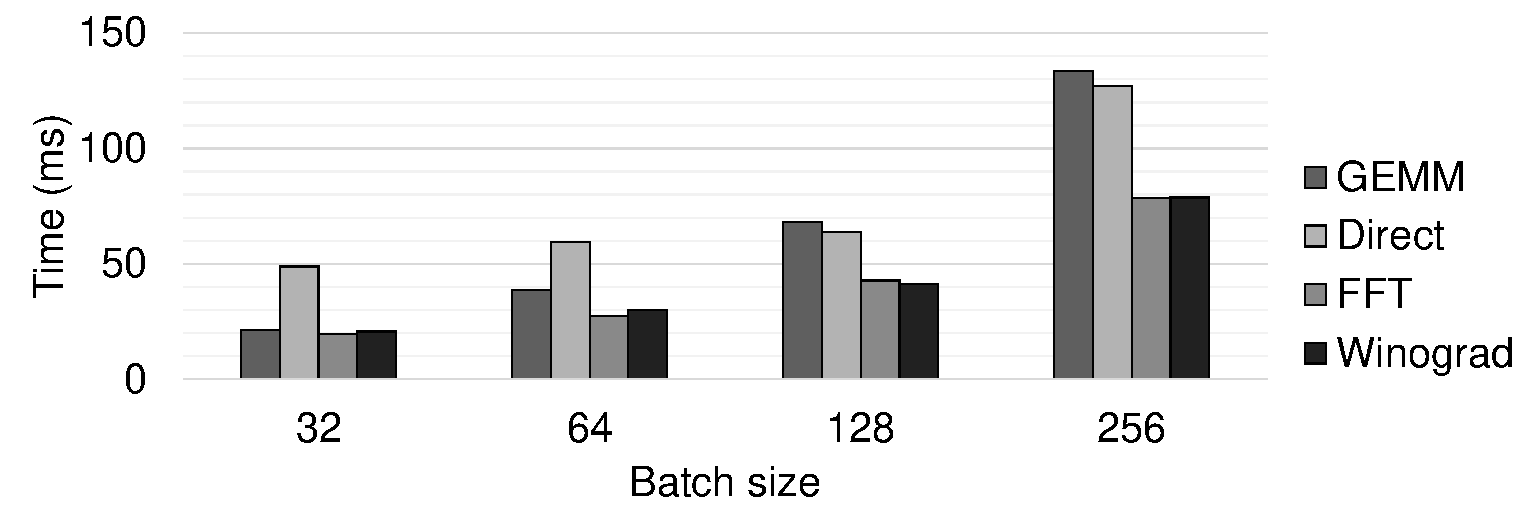
\includegraphics[width=.45\linewidth]{./figures/gpu_time_fwd}
  \label{fig_gpu_time_fwd}}
  \subfloat[Backpropagation execution time] {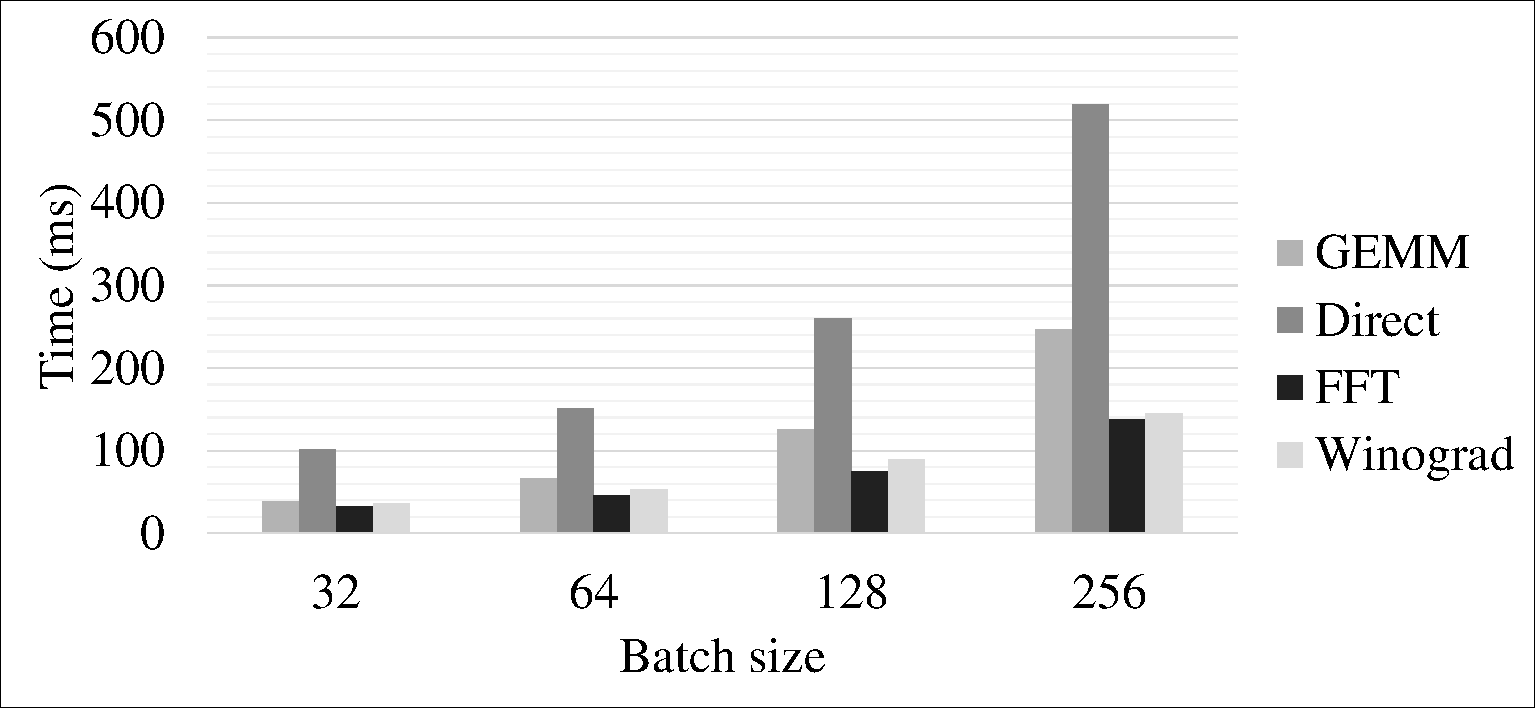
\includegraphics[width=.45\linewidth]{./figures/gpu_time_bwd}
  \label{fig_gpu_time_bwd}}
  \hfil
  \subfloat[Forward execution time from conv3 to conv5 layer] {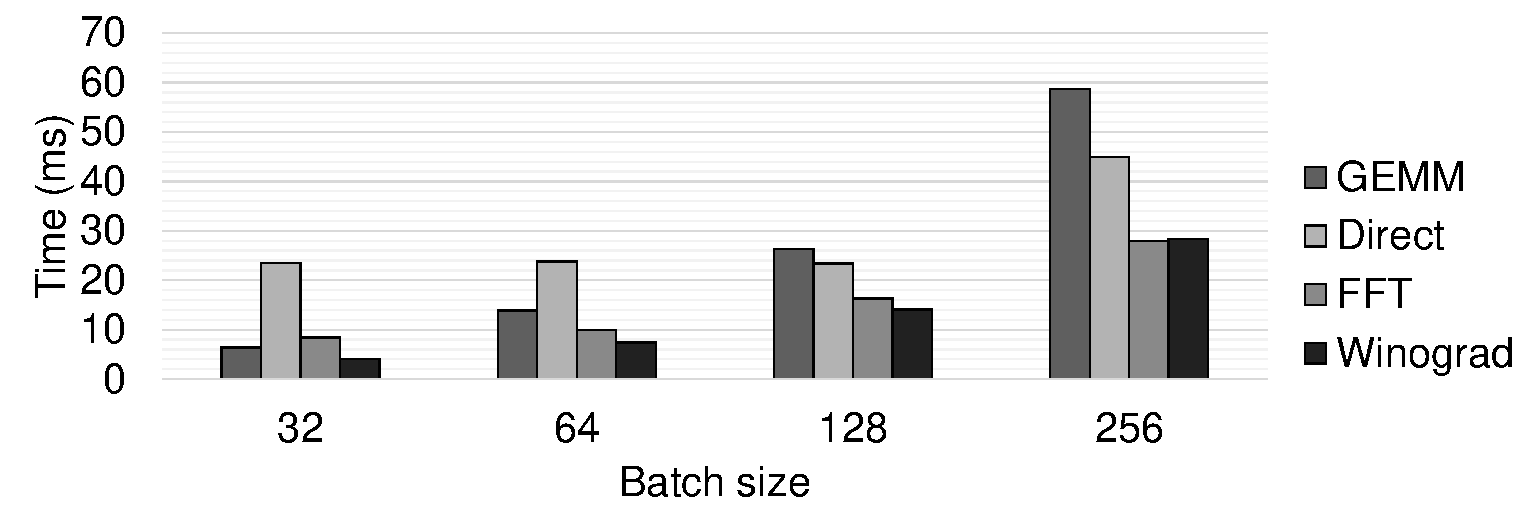
\includegraphics[width=.45\linewidth]{./figures/gpu_time_conv345}
  \label{fig_gpu_time_conv345}}
  \subfloat[Memory usage] {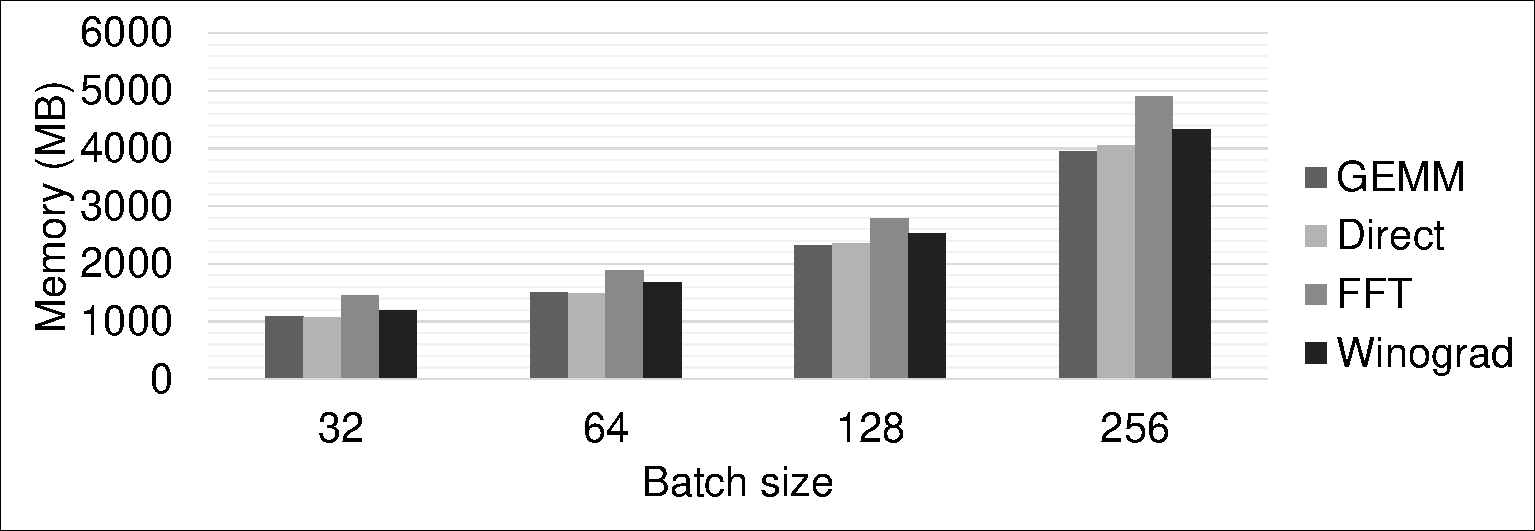
\includegraphics[width=.45\linewidth]{./figures/gpu_mem_kernels}
  \label{fig_gpu_mem}}
  \caption{Execution time and memory usage comparison of convolution kernels.}
  \label{fig_conv_time}
\end{figure*}

\begin{figure*}[!t]
  \centering
  \subfloat[Forward execution time] {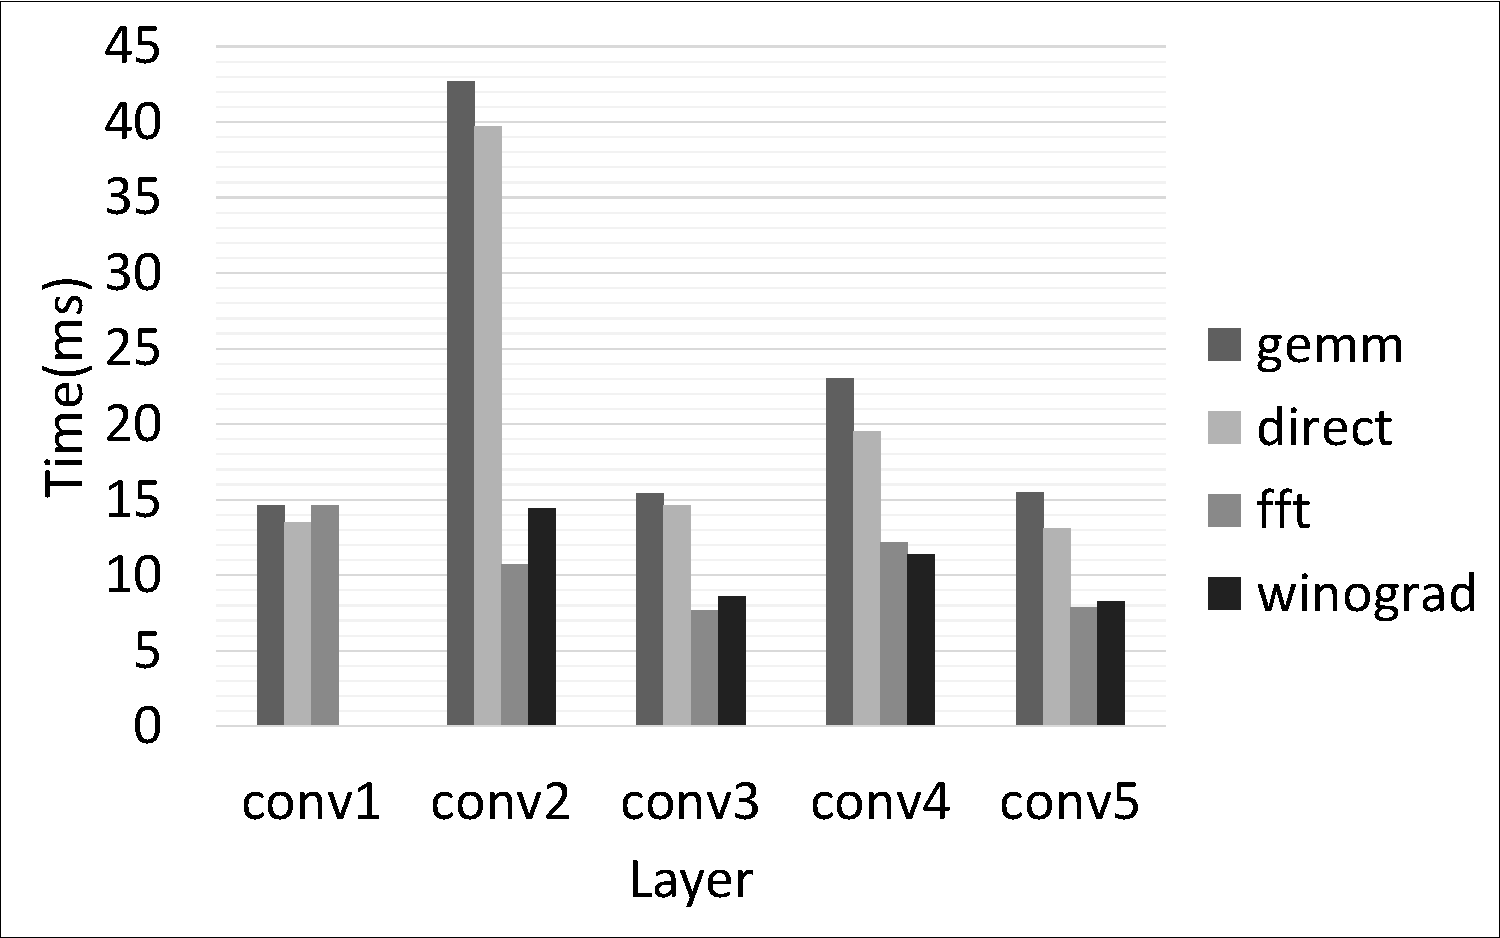
\includegraphics[width=.3\linewidth]{./figures/layerwise_fwd}
  \label{fig_layerwise_fwd}}
  \subfloat[Backward Data execution time] {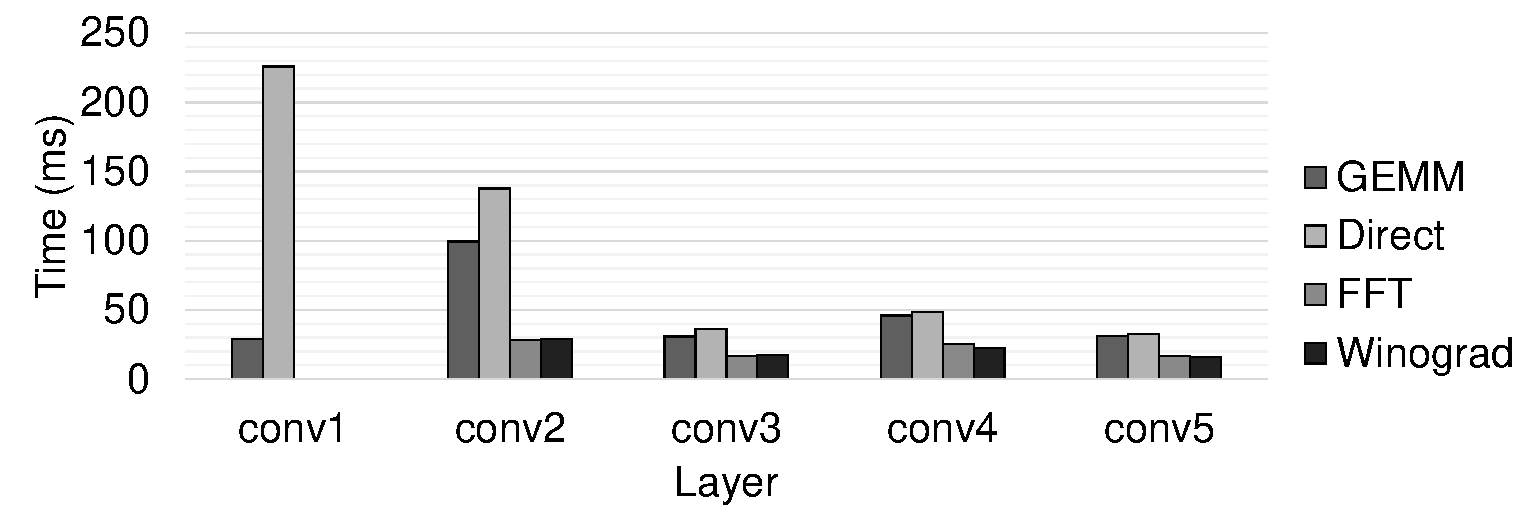
\includegraphics[width=.3\linewidth]{./figures/layerwise_bd}
  \label{fig_layerwise_bd}}
  \subfloat[Backward Filter execution time] {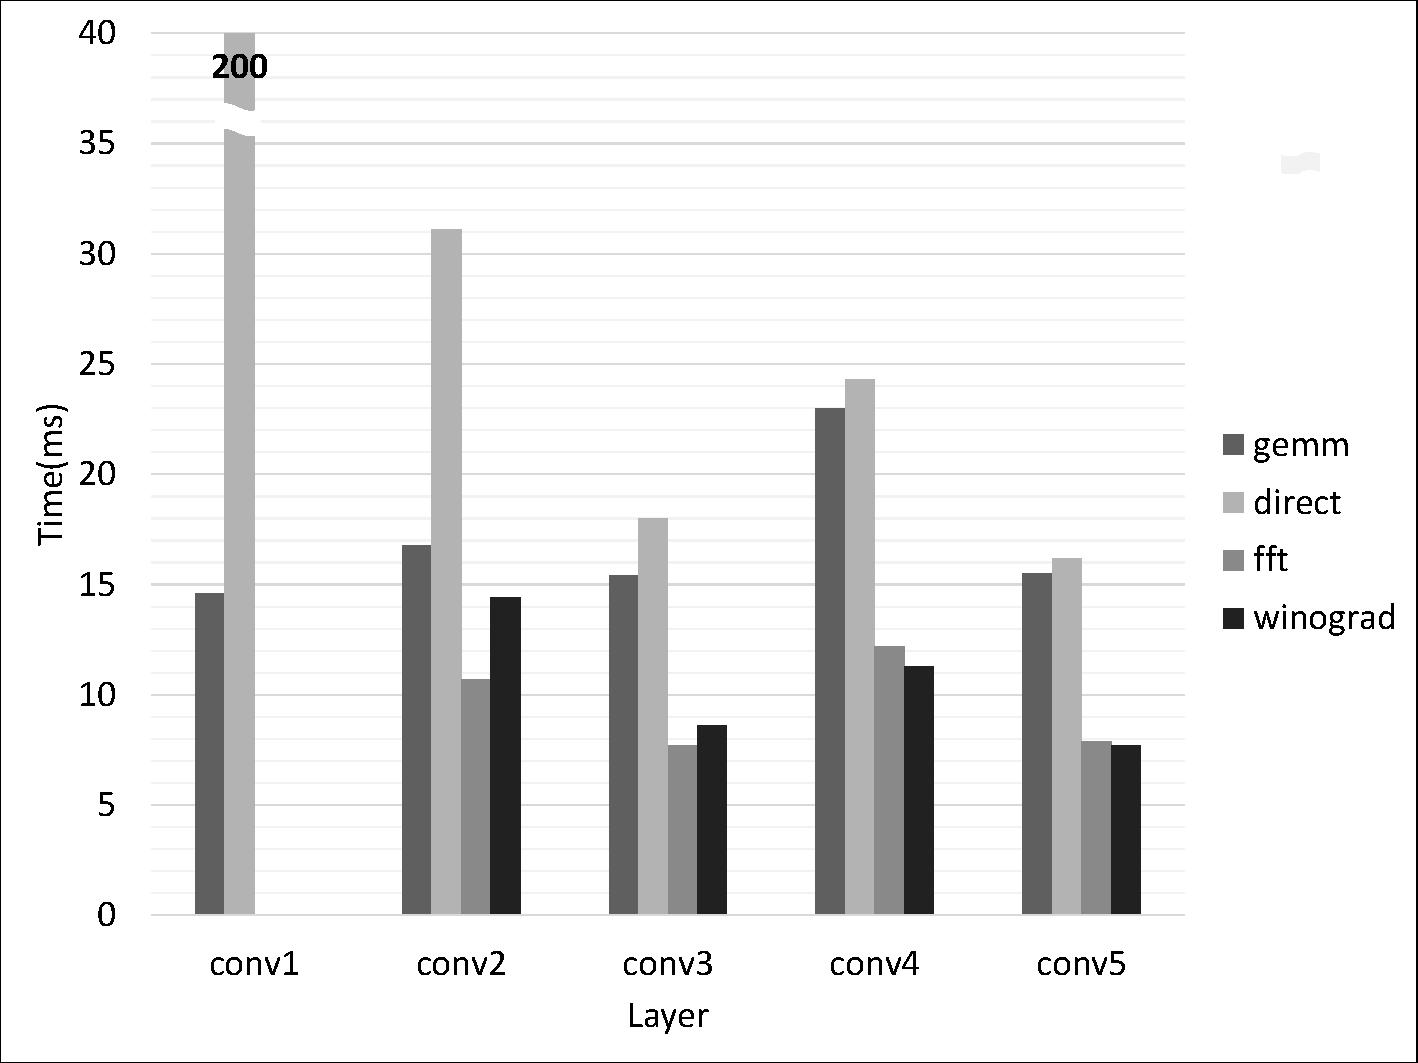
\includegraphics[width=.3\linewidth]{./figures/layerwise_bw}
  \label{fig_layerwise_bw}}
  \hfil
  \subfloat[Forward floating point operations count] {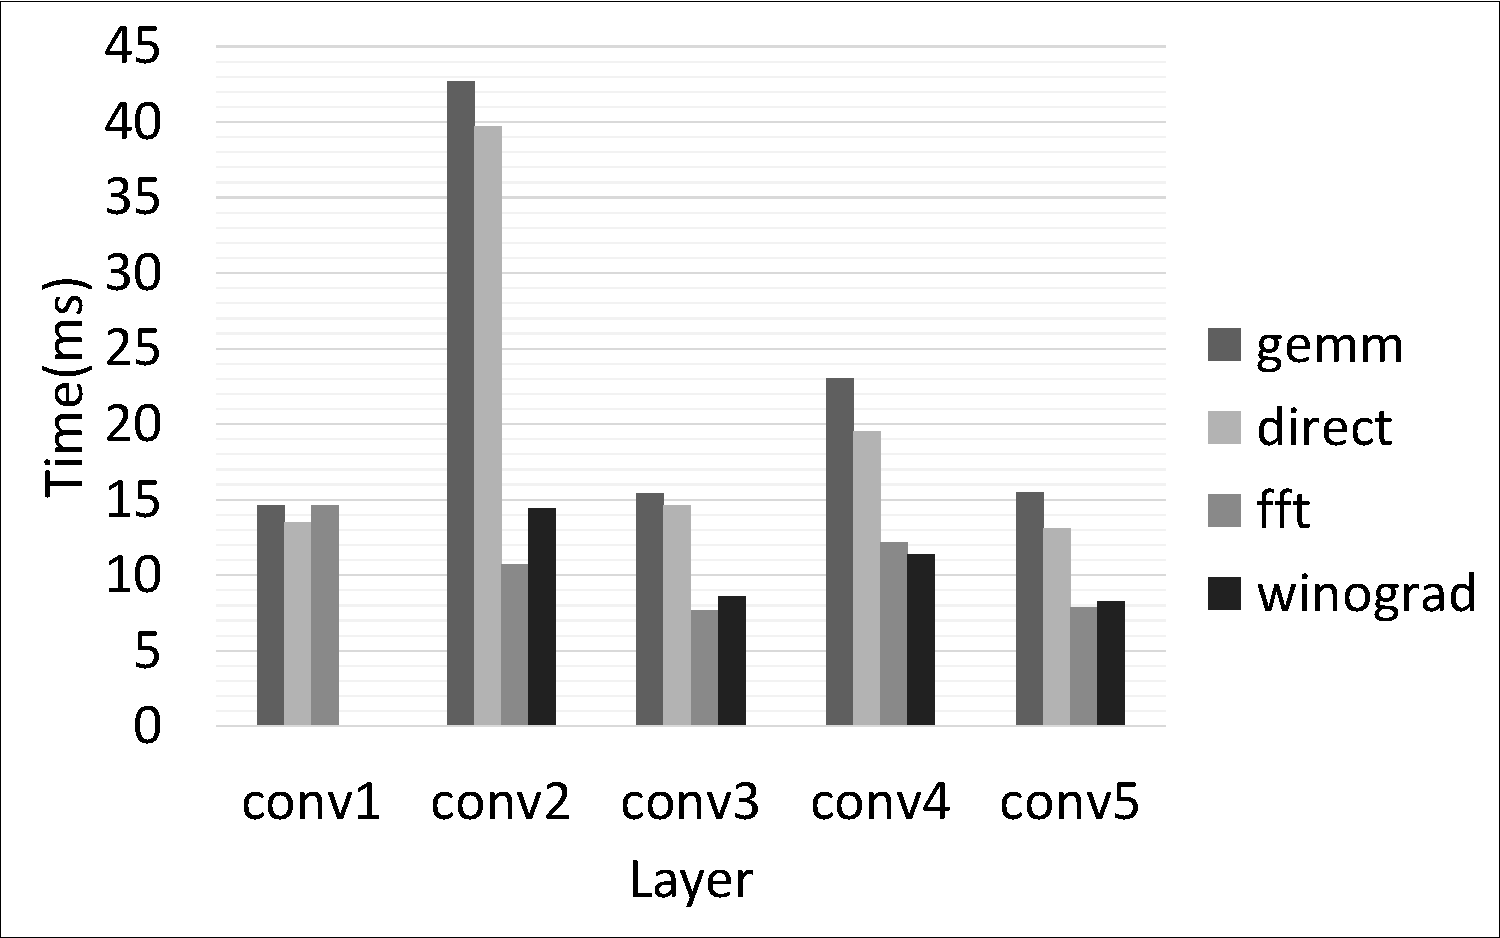
\includegraphics[width=.3\linewidth]{./figures/layerwise_fwd}
  \label{fig_layerwise_flop_count}}
  \subfloat[Forward Flops throughput] {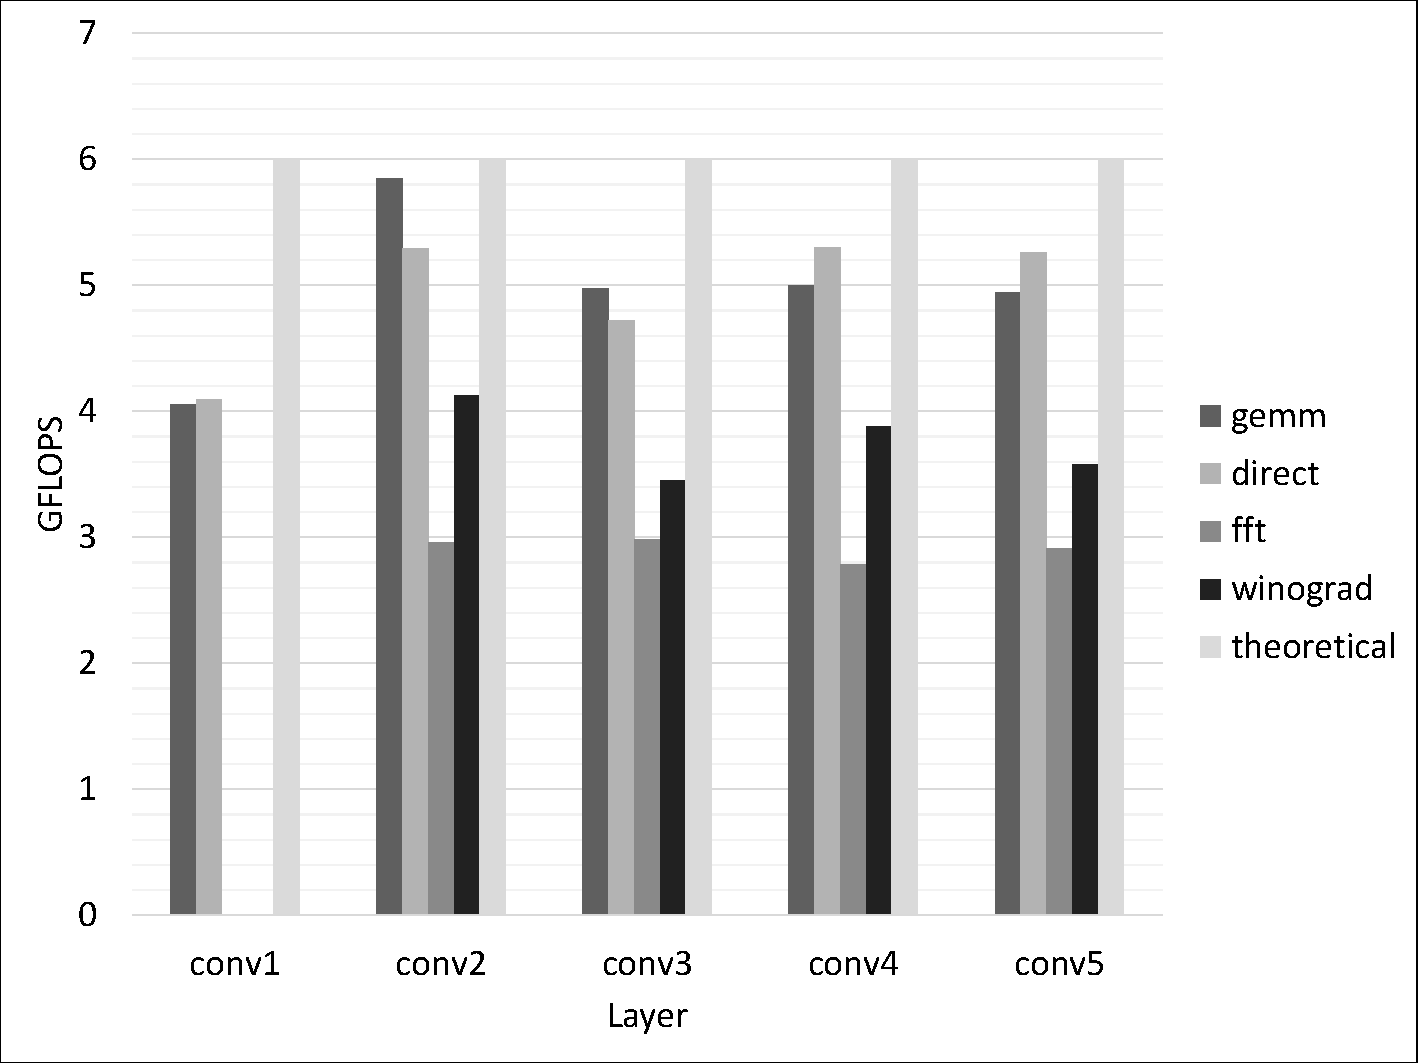
\includegraphics[width=.3\linewidth]{./figures/layerwise_flops_fwd}
  \label{fig_layerwise_flops_fwd}}
  \subfloat[Backward Flops throughput] {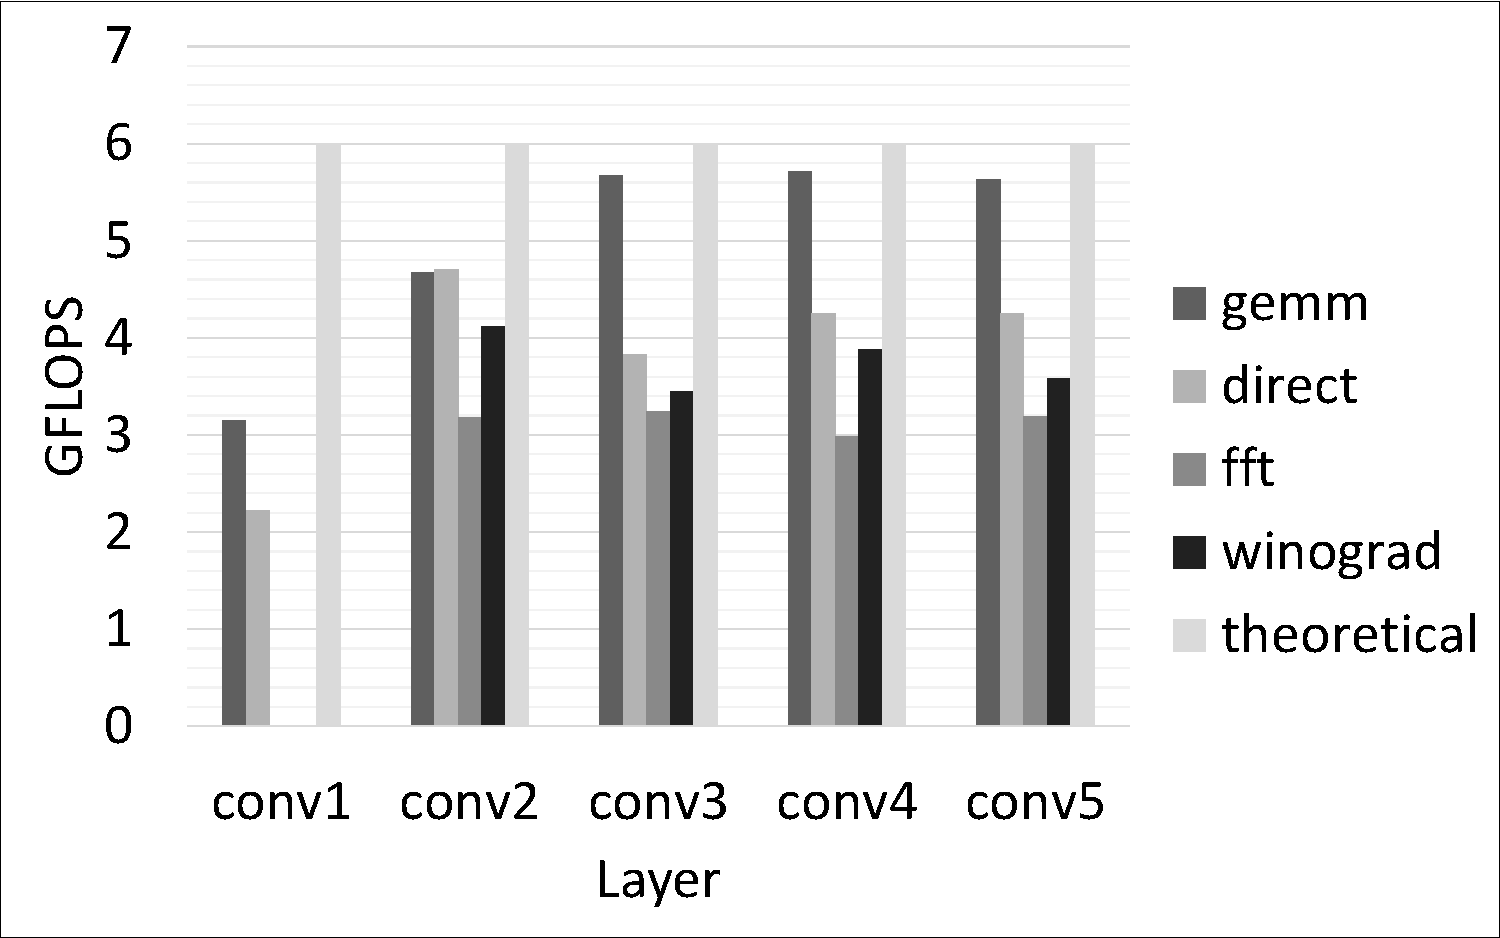
\includegraphics[width=.3\linewidth]{./figures/layerwise_flops_bd}
  \label{fig_layerwise_flops_bd}}
  \caption{Layerwise analysis of convolution kernels}
  \label{fig_layerwise}
\end{figure*}

FIg \ref{fig_conv_time} shows execution time comparisons between convolution kernels.
Winograd convolution and FFT convolution always perform better than direct or gemm convolution, due to smaller floating point operations required.
FFT has smallest operations count, makes it fastest among algorithms on big batch inputs.
However FFT scales bad on smaller batch sizes because it executes 5 kernels per each layer.
The forward propagation speed comparison on conv layer 3,4,5 on (f) of Fig \ref{fig_conv_time} clearly shows the differences.
Cuda-convnet scales bad when the batch size is smaller than 128 while GEMM convolutoin sclaes almost linearly.
Winograd performs better when the batch size is smaller than 64, where theoretical operations per each layer is around 20G operations.
Winograd kernels are more efficient when the sample width is even.
When we increase the sample width of conv layer 3,4,5 from 13 to 14, the execution time of Winograd kernels decrease by 10\%.

Number of floating point operations needed for forward propagation and backward propagation kernels are equal on the same layer.
Therefore, execution time of forward and backward propagation kernels are almost symmetric on most convolution algorithms.
However, backpropagation kernels of direct convolution takes more execution time than their forward counterparts.
Especially backward filter convolution on first convolution layer takes 200ms to execute, occupying 40\% of total training time.
The reason for the slow execution is low parallelism of kernels.
The backward direct convolution kernels have small thread numbers compared to other algorithms, generating 6 times smaller thread grid size.
The backward filter convolution for the first layer generates only 1024 threads, while Titan X has 3072 CUDA cores.




\subsection{Multi GPU analysis}

\begin{itemize}
  \item Support
  \item Scalability : proportion of data exchange
  \item Synchronization cost
\end{itemize}

\section{Discussion / Conclusion}

\begin{itemize}
  \item Summary of results
  \item Compare frameworks : Implementation difference
  \item Locate bottleneck / suggest possible optimization
  \item Limitation, future research
\end{itemize}

\section{Conclusions}


%\section*{Acknowledgment}

%The authors would like to thank...

\bibliographystyle{IEEEtran}
\bibliography{IEEEabrv,ispass17}
\nocite{*}

\end{document}
